% Kapittel 2 - Bakgrunn
\chapter{Bakgrunn}
\label{bakgrunn} % Bruk \ref{bakgrunn}, for å referere til kapittelet andre steder i oppgaven. 
%----------------------------------------------------------------------------------------
Dette kapittelet vil ta for seg nødvendig kunnskap om de viktigste hjelpemidler og verktøy brukt i arbeidet med denne oppgaven. Valgene vil bli presentert kort, men drøftingen av hvorfor de ulike valgene ble tatt, vil i hovedsak bli tatt opp i diskusjonskapittelet (kapittel \ref{diskusjon}).

\section{Generelt om applikasjonsutvikling for web}
Applikasjonsutvikling for web har hatt en kraftig økning de siste årene \cite{jsFrameworks}. En av årsakene er et ønske om å utvikle applikasjoner som skal kunne kjøres på alle enheter. Det er tidkrevende å utvikle applikasjoner for forskjellige operativsystemer, noe som fører til at flere og flere velger å satse på webapplikasjoner. Selv om man ikke får en applikasjon som er like tilpasset operativsystemet den kjører på, vil tida man sparer på utvikling og vedlikehold i mange tilfeller veie opp for dette.

\subsection{Rammeverk-muligheter i JavaScript}
JavaScript har etablert seg som det ledende språket for å utvikle web-applikasjoner og ble  stemt frem som et av de mest populære programmeringsspråkene i 2018 \cite{developerSurvey}. Det finnes i dag utallige frontend-rammeverk for web-utvikling i JavaScript; React, Angular, Vue.js, Ember, for å nevne noen. De to mest populære i 2018 var React og Angular \cite{jsFrameworks} og valget om hva som skulle brukes i denne applikasjonen stod hovedsakelig mellom disse to.

\subsection{Valg av JavaScript-rammeverk}
Selv om React og Angular er to rammeverk som ofte sammenlignes, er de bygget opp ganske forskjellig. Mens Angular er et fullverdig rammeverk, beskrives React best som et JavaScript-bibliotek. Angular blir derfor ofte sett på som vanskeligere å lære seg, på grunn av et stort antall muligheter og innebygde funksjoner. Størrelsen på Angular kan også øke innlastingstiden til en side noe, i forhold til sider skrevet i React \cite{angularvsreact}.

Å velge mellom disse to rammeverkene er ikke enkelt, men i dette prosjektet falt valget til slutt på Angular. Mer diskusjon rundt hvorfor og alternativene (i tillegg til React) som ble vurdert, vil bli diskutert senere i oppgaven (kapittel \ref{diskusjon}).

\section{Hva er Angular og hvordan fungerer det?}
Angular er en plattform og rammeverk som gjør det lettere å lage web-applikasjoner. Det er skrevet i TypeScript og har ulike maler, verktøy og integrerte metoder for å løse utviklingsutfordringer. Det har gode forutsetninger for å lage applikasjoner til datamaskin, mobil og nettbrett.

\subsection{Utvikle applikasjoner med Angular}
Det er et par ting man gjør for å sette opp et arbeidsmiljø og utvikle applikasjoner i Angular. Man kan installere Angular sitt eget kommandolinjeprogram ved bruk av Node Package Manager (NPM). Dette grensesnittet kan brukes til ulike ting, men er hovedsakelig brukt til å opprette prosjekter eller ferdige komponenter. Det har også mulighet til å gjennomføre oppgaver som testing og distribuering. For å teste applikasjonen kan man åpne den i nettleseren. Når en endring i filene blir oppdaget, vil serveren automatisk bygge applikasjonen på nytt og oppdatere siden \cite{AngularInBrowser}.

\subsection{Moduler i Angular}
Angular har sitt eget modulsystem kalt NgModules. NgModules er beholdere som beskriver hvordan de ulike delene av nettsiden skal settes sammen. De kan inneholde komponenter, tjenester, etc. Alle Angular-applikasjoner har en rotmodul som gjør at man har mulighet til å kjøre applikasjonen med en standard mal. I de fleste tilfeller legger man til flere typer moduler etter hvert. I Angular sorterer man inn i disse modultypene: funksjonsmoduler, rotmoduler, kjernemoduler, delte moduler og routing moduler. Det fins flere fordeler ved å splitte opp applikasjonen i ulike moduler: Det bidrar til en bedre kodestruktur, man kan bruke samme kode flere steder, og det fører også til en bedre ytelse \cite{angularModules}.

\subsection{Komponenter i Angular}
Komponentene i Angular bestemmer hvordan visningen av nettsiden skal fungere. Hver komponent definerer en klasse som inneholder både applikasjonsdata og logikk. Den henger sammen med en HTML-mal som viser innholdet. Et eksempel kan være: En nettside inneholder fire komponenter (en rot-, en navigasjonslinje-, en innholds- og en bunntekstkomponent). Om man trenger å gjøre endringer på innholdet til nettsiden, trenger man kun gjøre endringer inne i innholdskomponenten. Dette gjør at applikasjonen blir ryddigere og enkelere å endre på \cite{angularComponents}.

\subsection{Tjenester i Angular}
En viktig del av oppbygningen til en Angular-applikasjoner er tjenester. Tjenester i Angular er en bred kategori, men kan beskrives som definisjoner av verdier eller funksjoner applikasjonen trenger. En tjeneste er typisk en klasse med veldefinert formål som brukes i flere komponenter. Tjenester øker modulariteten og sjansen for gjenbruk i applikasjonen. En tjeneste kan brukes til å dele data mellom komponenter, men kan også bestå av funksjoner. Man kan for eksempel lage en tjeneste som validerer brukerinput. Ved å definere dette som en tjeneste, kan valideringen enkelt brukes i flere komponenter \cite{angularServices}.
\todo[inline]{Skrive noe om deling av data mellom komponenter}

\section{Designmønster i applikasjonsutvikling for web}
\subsection{Arkitekturmodellen Model View Controller}
Model View Controller (MVC) er en arkitektur som vanligvis blir brukt for å utvikle brukergrensesnitt og deler applikasjonen opp i tre ulike deler. MVC-arkitekturen deler opp store komponenter, og målet er å kunne gjenbruke kode flere ulike steder \cite{MVC_uses}. Denne arkitekturen har i senere tid blitt svært populær for designing av nett- og mobilapplikasjoner. Populære programmeringsspråk som Java, C\#, Python, Ruby og PHP har alle MVC-rammeverk som er brukt i webutvikling. 

\subsubsection{Komponentene i Model View Controller}
Slik som med andre designmønster så er MVC kun kjernen av arkitekturen. Det finnes nok mange MVC arkitekturer som kan skille seg fra den generelle forklaringen under, men den gir et godt bilde på grunnprinsippet \cite{MVC_coreArc}.
\begin{itemize}
    \item Modellen (model) er den sentrale komponenten i mønsteret. Det er applikasjonens dynamiske datastruktur, uavhengig av brukergrensesnittet. Modellen håndterer data, logikk og regler i applikasjonen.
    \item En visning (view) kan være en fremvisning av informasjon. Det er mulig å ha flere visninger for samme informasjon. For eksempel kan visningen være både en tabell og en graf som viser til samme data. 
    \item Kontrolleren (controller) tar brukerinput og konverterer det til kommandoer for enten modellen eller visningen \cite{MVC_components}. 
\end{itemize}

\subsubsection{Relasjonene mellom komponentene i Model View Controller}
I tillegg til å dele applikasjonen inn i tre komponenter, så bestemmer også MVC-designet relasjonene mellom dem. 
\begin{itemize}
    \item Modellen har ansvaret for å håndtere all data i applikasjonen. Den mottar brukerinput fra kontrolleren.
    \item Visningen presenterer modellen i et spesifikt format.
    \item Kontrolleren responderer på brukerinputen og utfører operasjoner på objektene fra datamodellen. Kontrolleren mottar inputen før den eventuelt validerer den og så sender den videre til modellen \cite{MVC_relations}.
\end{itemize}
\begin{figure}[ht]
    \centering
    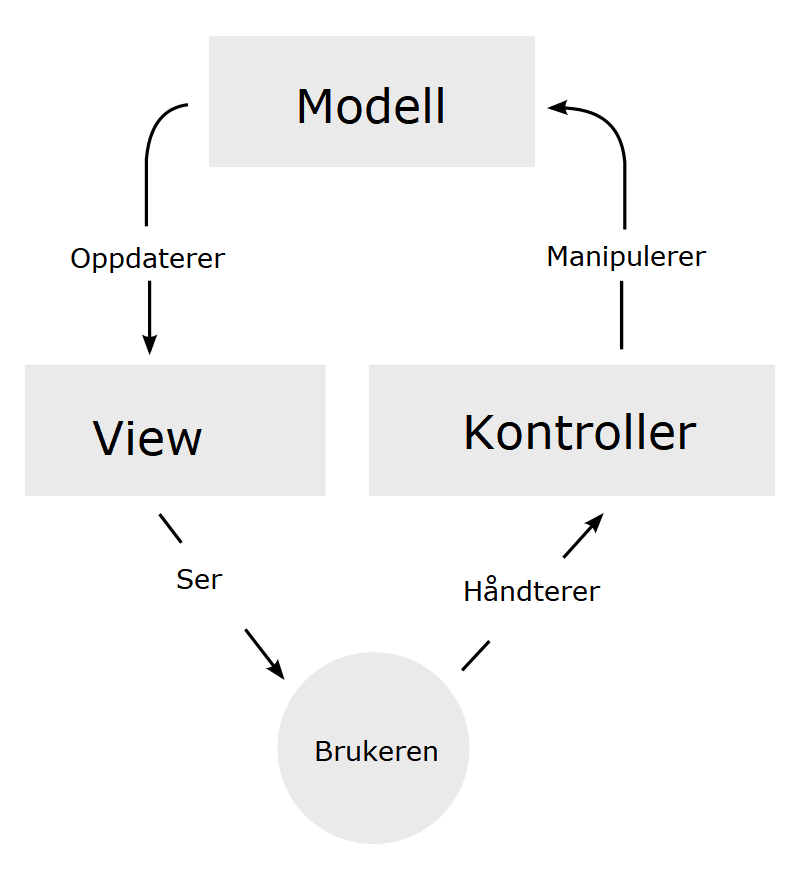
\includegraphics[width=0.7\textwidth]{Figurer/MVC_prosess.png}
    \caption{Relasjoner mellom komponentene i en Model View Controller arkitektur}
    \label{fig:mvc_relations}
\end{figure}

\subsubsection{Fordeler og ulemper med Model View Controller}
Fordeler:
\begin{itemize}
    \item Samarbeid under utvikling: Flere utviklere kan arbeide samtidig på modellen, kontrolleren og visningene. 
    \item Enklere å modifisere: Siden de ulike komponentene har egne ansvarsområder, så er det lettere å gjøre endringer på applikasjonen senere.
    \item Modellen kan ha flere visninger
\end{itemize}
Ulempe:
\begin{itemize}
    \item Omfattende: Rammeverket kan være vanskelig å forstå fordi det introduserer mange nye begrep, sammenhenger og relasjoner som må læres.
\end{itemize}
\subsection{Avhengighetsinjeksjons-mønster} % Depenedecy injection som mønster

\begin{wrapfigure}[9]{r}{0.35\textwidth} % [antall linjer]{float}{bredde}
    \centering
    
\includegraphics[width=0.3\textwidth]{Figurer/Dependency_injection.png}
    \caption{Tjeneste brukt i en komponent \cite{angularDI}}
    \label{fig:di}
\end{wrapfigure}

Avhengighetsinjeksjon (en: dependecy injection) er et designmønster hvor klasser får avhengigheter fra eksterne kilder istedenfor å opprette dem selv. Dette gjør at flere klasser kan dele samme ressurs og på den måten øker man modulariteten i applikasjonen \cite{whatIsDI}.

Et typisk eksempel hvor avhengighetsinjeksjon blir brukt i Angular, er tjenester. En tjeneste defineres med en spesifikk funksjon som alle komponentene kan abonnere på hvis de trenger denne (som vist i figur \ref{fig:di}).

\section{Viktige tillegg brukt i applikasjonen}
%I dette prosjektet er det brukt noen tilleggsverktøy for å gjøre utviklingen enklere og mer oversiktlig. De viktigste av disse vil bli beskrevet i dette delkapittelet.

\subsection{Stilsetting med Bootstrap}
Bootstrap er et verktøy som brukes for å enklere stilsette nettsider. Hovedformålet er å spare tid, samt at man lettere får en gjennomført stil på siden. Bootstrap gir deg tilgang til ferdiglagde til knapper, skjema, navigasjonslinjer og andre grensesnittkomponenter. Komponentene er laget for å kunne justere seg automatisk og nettsiden vil derfor få ett responsivt design som tilpasser seg størrelsen på enheten din. Figur \ref{fig:bootstrap_layout} viser et eksempel på hvordan innholdet på siden kan justere seg avhengig av størrelsen.

\begin{figure}[ht]
    \centering
    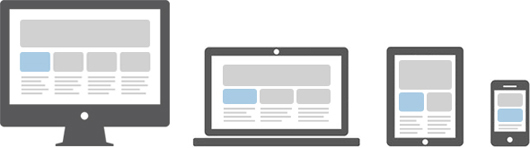
\includegraphics[width=\textwidth]{Figurer/Bootstrap_layout.jpg}
    \caption{Bootstrap oppsett. Innhold justeres etter skjermstørrelse \cite{bootstrap_figur}}
    \label{fig:bootstrap_layout}
\end{figure}

\subsection{Graftegning med Chart.js}
Grafene i denne applikasjonen er tegnet ved hjelp av Chart.js. Dette er et «open source» JavaScript-bibliotek som gjør tegning av grafer enklere. Verktøyet lager en dynamisk graf og vil automatisk sørge for at grafen ser bra ut og at navn er lesbare. Hvis man endrer oppsettet og gir mer rom til grafen i applikasjonen, vil den automatisk utvide størrelsen. Chart.js gjør også tilpassing av utseende på grafen enkelt (e.g. farge, akse-beskrivelse). For å kunne bruke Chart.js biblioteket i Angular på en effektiv måte, ble utvidelsen Ng2-charts brukt. Man får da tilgang til Chart.js biblioteket som en komponent i Angular-applikasjonen og kan enkelt tegne grafer på lignende måte som man ville gjort på en vanlig nettside ved hjelp av HTML/JS.

\section{Bruken av versjonskontroll}
For å ha kontroll på koden og muligheten til å rulle tilbake endringer hvis det skulle oppstå problemer, er bruken av versjonskontroll viktig i et slikt prosjekt. I dette prosjektet hadde man to hovedgrener: «Master» og «Dev». Master-grenen inneholdt siste stabile versjonen av applikasjonen og ble oppdatert regelmessig (fra dev-grenen) gjennom hele perioden. Dev-grenen ble brukt til å implementere ny funksjonalitet, og dette førte til at den inneholdt funksjoner som ikke alltid var skikkelig testet. For å effektivisere bruken av versjonskontrollen, ble det ofte opprettet nye grener ut fra dev-grenen. Dette ble gjort slik at man kunne arbeide fritt, uten at det førte til problemer i dev. Etter at en funksjonalitet var ferdig implementert i den nye grenen, ble den slått sammen med dev igjen.

For å holde oversikt over oppgaver, forbedringer og feil i prosjektet/koden ble «Github Issues» brukt \cite{githubIssues}. Dette ble brukt som et verktøy hvor man raskt kunne se hva som måtte gjøres, og samtidig kunne man også se tilbake på ting som hadde blitt gjort. Nye punkter ble lagt til etterhvert som prosjektet utviklet seg og markert ferdige når de var implementert. 

\section{Oppsummering av kapittelet}
Angular, sammen med tillegg som Bootstrap og Chart.js, har blitt brukt til å utvikle denne applikasjonen. Hvordan disse verktøyene fungerer, samt hvordan versjonskontroll har hjulpet i utviklingsprosessen, har i dette kapittelet blitt beskrevet. Målet har vært å gi litt bakgrunnskunnskap for å enklere kunne beskrive konstruksjonen av applikasjonen (kapittel \ref{konstruksjon}). 
\todo[inline]{Legg til litt om designmønster i oppsummeringen}
